% ============================================================
%  PRÉSENTATION BEAMER — État d'avancement du mémoire
%  Auteur  : NDZESSA AVELE BRUNO LANDRY
%  Titre   : Plateforme gouvernementale pour la cartographie
%             et la mise en relation des besoins des entreprises
%  ENSPM — Université de Maroua | 2025/2026
%  Version enrichie : ajout section "Présentation de l'application"
%  + section "Limites et perspectives" + corrections mineures
% ============================================================

\documentclass[aspectratio=169, 10pt]{beamer}

% ------------------------------------------------------------
%  THÈME DE BASE
% ------------------------------------------------------------
\usetheme{Madrid}
\usecolortheme{default}
\usepackage{tikz}
\usetikzlibrary{positioning}
\usetikzlibrary{shapes.geometric}
\usepackage{graphicx}
\usepackage{float}
\usepackage{subcaption} % Requis pour les sous-figures

% ------------------------------------------------------------
%  ENCODAGE & LANGUE
% ------------------------------------------------------------
\usepackage[utf8]{inputenc}
\usepackage[T1]{fontenc}
\usepackage[french]{babel}
\usepackage{csquotes}

% ------------------------------------------------------------
%  POLICES
% ------------------------------------------------------------
\usepackage{lmodern}
\usepackage{microtype}

% ------------------------------------------------------------
%  MATHS
% ------------------------------------------------------------
\usepackage{amsmath, amssymb}
\usepackage{bm}

% ------------------------------------------------------------
%  GRAPHIQUES & TABLEAUX
% ------------------------------------------------------------
\usepackage{graphicx}
\usepackage{booktabs}
\usepackage{tabularx}
\usepackage{multirow}
\usepackage{colortbl}
\usepackage{tikz}
\usetikzlibrary{shapes, arrows.meta, positioning, calc}

% ------------------------------------------------------------
%  COULEURS — reprises du mémoire
% ------------------------------------------------------------
\definecolor{primary}{RGB}{0, 51, 102}
\definecolor{secondary}{RGB}{0, 102, 153}
\definecolor{accent}{RGB}{200, 50, 50}
\definecolor{lightgray}{RGB}{245, 245, 245}
\definecolor{darkgray}{RGB}{80, 80, 80}
\definecolor{successgreen}{RGB}{34, 139, 34}

% ------------------------------------------------------------
%  PERSONNALISATION DU THÈME BEAMER
% ------------------------------------------------------------
\setbeamercolor{palette primary}{bg=primary, fg=white}
\setbeamercolor{palette secondary}{bg=secondary, fg=white}
\setbeamercolor{palette tertiary}{bg=primary!80, fg=white}
\setbeamercolor{palette quaternary}{bg=primary, fg=white}
\setbeamercolor{structure}{fg=primary}
\setbeamercolor{section in toc}{fg=primary}
\setbeamercolor{frametitle}{bg=primary, fg=white}
\setbeamercolor{title}{bg=primary, fg=white}
\setbeamercolor{block title}{bg=primary, fg=white}
\setbeamercolor{block body}{bg=primary!8, fg=black}
\setbeamercolor{block title alerted}{bg=accent, fg=white}
\setbeamercolor{block body alerted}{bg=accent!8, fg=black}
\setbeamercolor{block title example}{bg=successgreen!80, fg=white}
\setbeamercolor{block body example}{bg=successgreen!8, fg=black}
\setbeamercolor{itemize item}{fg=primary}
\setbeamercolor{itemize subitem}{fg=secondary}
\setbeamercolor{enumerate item}{fg=primary}

\setbeamerfont{frametitle}{series=\bfseries}
\setbeamerfont{title}{series=\bfseries, size=\large}
\setbeamerfont{block title}{series=\bfseries}

% Navigation simplifiée
\setbeamertemplate{navigation symbols}{}
\setbeamertemplate{footline}{
    \leavevmode
    \hbox{%
        \begin{beamercolorbox}[wd=.33\paperwidth, ht=2.25ex, dp=1ex, center]{palette primary}
            \usebeamerfont{author in head/foot}\insertshortauthor
        \end{beamercolorbox}%
        \begin{beamercolorbox}[wd=.34\paperwidth, ht=2.25ex, dp=1ex, center]{palette secondary}
            \usebeamerfont{title in head/foot}\insertshorttitle
        \end{beamercolorbox}%
        \begin{beamercolorbox}[wd=.33\paperwidth, ht=2.25ex, dp=1ex, center]{palette primary}
            \usebeamerfont{date in head/foot}
            \insertframenumber{} / \inserttotalframenumber
        \end{beamercolorbox}%
    }
    \vskip0pt%
}

% Séparateur de section
\AtBeginSection[]{
    \begin{frame}
        \vfill
        \centering
        \begin{beamercolorbox}[sep=12pt, center, rounded=true, shadow=true]{palette primary}
            \usebeamerfont{title}
            \insertsectionhead\par
        \end{beamercolorbox}
        \vfill
    \end{frame}
}

% ------------------------------------------------------------
%  COMMANDE UTILITAIRE — emplacement de capture d'écran
%  (à remplacer par \includegraphics[width=..]{fichier.png}
%   dès que vous aurez vos images réelles)
% ------------------------------------------------------------
\newcommand{\screenshotplaceholder}[3][7cm]{%
    \begin{tikzpicture}
        \node[draw=darkgray, dash pattern=on 4pt off 3pt, thick,
              fill=lightgray!60, minimum width=#1, minimum height=#2,
              align=center, font=\itshape\footnotesize, text=darkgray,
              rounded corners=3pt] {#3};
    \end{tikzpicture}%
}

% ============================================================
%  MÉTADONNÉES
% ============================================================
\title[Cartographie des besoins des entreprises camerounaises par analyse multidimensionnelle et développement d'une plateforme gouvernementale de mise en relation]{%
    Cartographie des besoins des entreprises camerounaises par analyse multidimensionnelle et développement d'une plateforme gouvernementale de mise en relation}

\subtitle{Présentation en vue de l'obtention du Diplôme d'Ingénieur en Data Sciences}

\author[NDZESSA AVELE Bruno Landry]{%
    \textbf{NDZESSA AVELE BRUNO LANDRY}\\
    \small Matricule : 21D0180EP}

\institute[ENSPM — Maroua]{%
    École Nationale Supérieure Polytechnique de Maroua\\
    Département d'Informatique et Télécommunications\\[4pt]
    \small Directeur : Pr Mohamadou Alidou\\
    Encadreur académique : Pr Kaladzavi\\
    Encadreur professionnel : M. Abdoulaziz Junmbe
    }

\date{Année académique 2025 / 2026}

% ============================================================
%  DOCUMENT
% ============================================================
\begin{document}

% -----------------------------------------------------------
%  DIAPO 1 — PAGE DE TITRE
% -----------------------------------------------------------
\begin{frame}[plain]
    \titlepage
\end{frame}

% -----------------------------------------------------------
%  DIAPO 2 — PLAN
% -----------------------------------------------------------
\begin{frame}{Plan de la présentation}
    \tableofcontents[hideallsubsections]
\end{frame}

% ============================================================
\section{Introduction Générale}
\begin{frame}{Contexte}
    \begin{itemize}
        \item Le secteur privé est un moteur essentiel de la production de richesse et de la création de valeur ajoutée ;
        \item La SND30 fixe au Cameroun l'objectif d'un secteur privé fort, pilier de la croissance économique ;
        \item Des réformes ont été engagées et des indicateurs de croissance définis ;
        \item L'évaluation à mi-parcours de la SND30 révèle une économie résiliente, mais encore loin des ambitions fixées ;
        \item Le MINEPAT lance une enquête sur les besoins des entreprises et instruit la création d'une plateforme numérique de mise en relation.
    \end{itemize}
\end{frame}

\begin{frame}{Problématique}
    \begin{enumerate}
        \item Le secteur privé est incontournable pour la croissance économique, mais rencontre au Cameroun d'énormes difficultés ;
        \item Soutenir sa contribution suppose que l'administration aide les entreprises à lever les contraintes qui freinent leur activité ;
        \item Plusieurs initiatives ont déjà été engagées en ce sens, avec des résultats peu concluants ;
        \item Une enquête de recensement des besoins des entreprises est lancée par le MINEPAT en 2025.
    \end{enumerate}
    \vspace{6pt}
    \begin{alertblock}{Question centrale}
        Quels profils de besoins existent dans l'économie camerounaise, et comment y répondre au travers d'une plateforme numérique de mise en relation ?
    \end{alertblock}
\end{frame}

\begin{frame}{Objectifs}
    Il sera question de présenter les résultats de l'analyse des données de l'enquête MINEPAT sur la cartographie des entreprises, puis de proposer une application de mise en relation basée sur les besoins et offres exprimés.
    \vspace{4pt}
    \textbf{Objectifs spécifiques :}
    \begin{itemize}
        \item Effectuer des analyses descriptives sur les données épurées ;
        \item Utiliser les méthodes d'analyse dimensionnelle (ACM, CAH, AFD) pour synthétiser les données et proposer des profils de besoins ;
        \item Modéliser et développer une application de mise en relation des entreprises.
    \end{itemize}
\end{frame}

\begin{frame}{Méthodes utilisées}
    \textbf{Analyse des données :}
    \begin{itemize}
        \item Statistique descriptive univariée (graphiques de proportion) ;
        \item Statistique descriptive bivariée (test du $\chi^2$, $V$ de Cramér) ;
        \item Analyse des Correspondances Multiples — représenter modalités et entreprises dans un espace de dimension réduite ;
        \item Classification Ascendante Hiérarchique — construire des classes à partir des coordonnées de l'ACM (critère de Ward) ;
        \item Analyse Factorielle Discriminante — valider et prédire l'appartenance des entreprises aux classes.
    \end{itemize}
    \textbf{Conception de la plateforme :}
    \begin{itemize}
        \item Modélisation dimensionnelle;
        \item Implémentation via l'ORM Django ;
        \item Définition des routes et vues ;
        \item Tests de l'application.
    \end{itemize}
\end{frame}

\section{Définition des concepts et état de l'art}

\begin{frame}{Cartographie des besoins des entreprises}
    La Banque Mondiale définit les besoins des entreprises comme l'ensemble des contraintes qui, une fois levées, permettraient d'améliorer significativement leur productivité et leur capacité à croître.

    La cartographie des besoins est un processus systématique de collecte, d'organisation et de représentation sectorielle des contraintes exprimées par les unités économiques d'un territoire donné.
\end{frame}

\begin{frame}{Mise en relation}
    La mise en relation des entreprises renvoie au mécanisme par lequel deux ou plusieurs unités économiques sont amenées à se connaître, à échanger sur leurs capacités et besoins respectifs, et à explorer les conditions d'une collaboration mutuellement bénéfique.
    \vspace{4pt}
    \textbf{Mécanismes existants :}
    \begin{itemize}
        \item Plateformes B2B (Amazon, Facebook Marketplace, Alibaba) ;
        \item Bourse de sous-traitance et de partenariat ;
        \item Partenariats contractuels directs.
    \end{itemize}
\end{frame}

\begin{frame}{Études antérieures sur les besoins des entreprises}
    \begin{itemize}
        \item \textbf{Enquête GECAM (2019)} : 57\% des entreprises du groupement rencontrent des difficultés ; la fiscalité est le principal frein — instabilité du système fiscal (72\%), pénalités et amendes (66\%), niveau d'imposition (61\%), multiplicité des contrôles (59\%) ;
        \item \textbf{Stratégie de développement du secteur industriel} : la valeur ajoutée manufacturière stagne à 14,08\% du PIB en 2015 (contre 28,6\% en Thaïlande, 24\% en Malaisie) ; 90\% des entreprises locales sont des TPE/PME ; des projets structurants (FABER, 8~000~km de voies ferrées) sont envisagés ;
        \item \textbf{Enquête MINEPAT sur le climat des affaires} : 91\% des chefs d'entreprise jugent trop élevés les coûts liés aux taux d'intérêt, assurances et courtage ; l'accès aux facteurs de production et l'état des infrastructures routières sont des freins majeurs.
    \end{itemize}
\end{frame}

\begin{frame}{Outils existants de mise en relation}
    La mise en relation des entreprises s'apparente à un système de recommandation. La littérature en distingue trois grandes familles :
    \begin{itemize}
        \item \textbf{Filtrage basé sur le contenu} : propose des éléments présentant des attributs similaires à ceux avec lesquels l'utilisateur a déjà interagi ;
        \item \textbf{Filtrage collaboratif} : exploite les comportements collectifs des utilisateurs pour inférer des affinités ;
        \item \textbf{Systèmes à base de connaissances} : font correspondre les contraintes d'un utilisateur aux caractéristiques des éléments disponibles — \textit{c'est l'approche retenue pour notre plateforme}.
    \end{itemize}
\end{frame}

\section{Présentation des résultats de l'analyse des données de l'enquête}

\begin{frame}{Source des données : enquête MINEPAT 2025}
    \begin{columns}[T]
        \begin{column}{0.38\textwidth}
            \begin{block}{Dispositif de collecte}
                \begin{itemize}
                    \item Enquête sur les besoins des entreprises ;
                    \item Outil de collecte : plateforme numérique pour la centralisation des données ;
                    \item Couverture : toutes les régions du Cameroun ;
                    \item Stockage : base MySQL, deux tables (identifications et besoins).
                \end{itemize}
            \end{block}
        \end{column}
        \begin{column}{0.58\textwidth}
            \begin{block}{Variables descriptives et besoins retenus}
                \begin{enumerate}
                    \item Description : raison sociale, région, taille, statut, secteur d'activité, date de début d'activité ;
                    \item Besoins retenus : intrants, financement, emballages, transport, appui aux entreprises, équipements, innovation/recherche ;
                    \item Jonction réalisée entre les deux tables ;
                    \item Une ligne = une entreprise ; présence d'un besoin codée Oui/Non.
                \end{enumerate}
            \end{block}
        \end{column}
    \end{columns}
\end{frame}

\begin{frame}{Résultat de l'analyse descriptive}
    \footnotesize
    \begin{figure}[H]
        \centering
        \begin{subfigure}[b]{0.32\textwidth}
            \centering
            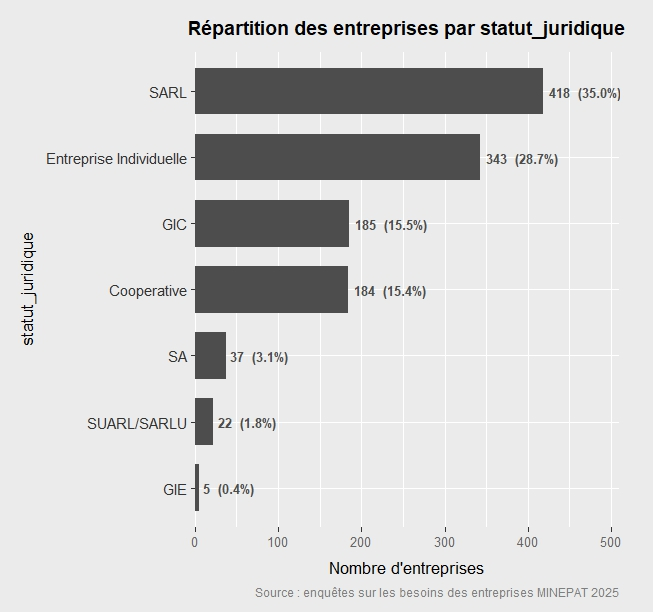
\includegraphics[width=\textwidth]{statut.jpeg}
            \caption{Répartition des entreprises par statut juridique}
            \label{fig:sous_fig_a}
        \end{subfigure}
        \hfill
        \begin{subfigure}[b]{0.32\textwidth}
            \centering
            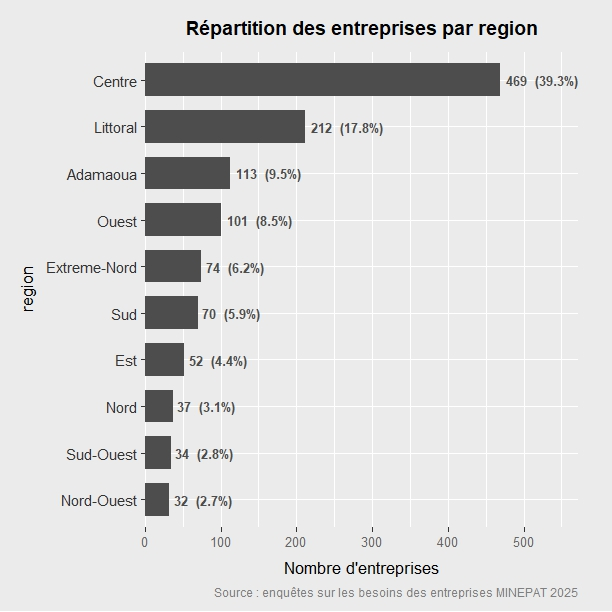
\includegraphics[width=\textwidth]{repartition_region.jpeg}
            \caption{Répartition des entreprises par région}
            \label{fig:sous_fig_b}
        \end{subfigure}
        \hfill
        \begin{subfigure}[b]{0.32\textwidth}
            \centering
            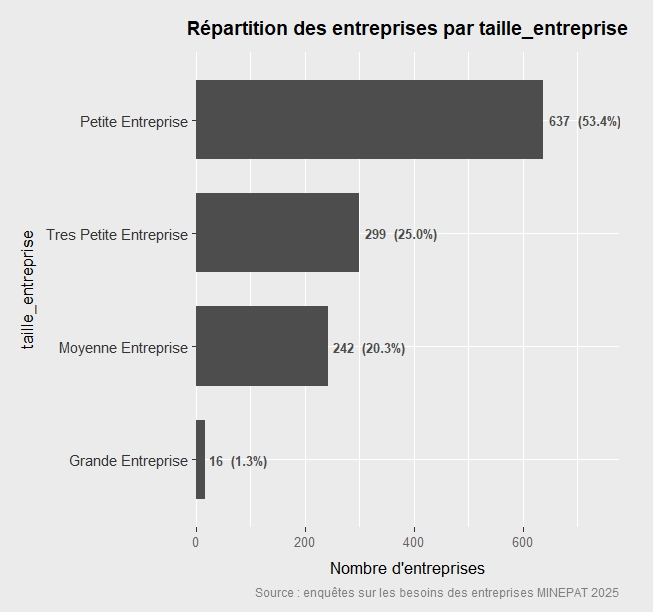
\includegraphics[width=\textwidth]{repartition_taille.jpeg}
            \caption{Répartition des entreprises par taille}
            \label{fig:sous_fig_c}
        \end{subfigure}
    \end{figure}
\end{frame}

\begin{figure}[H]
    \begin{subfigure}[b]{0.42\textwidth}
        \centering
        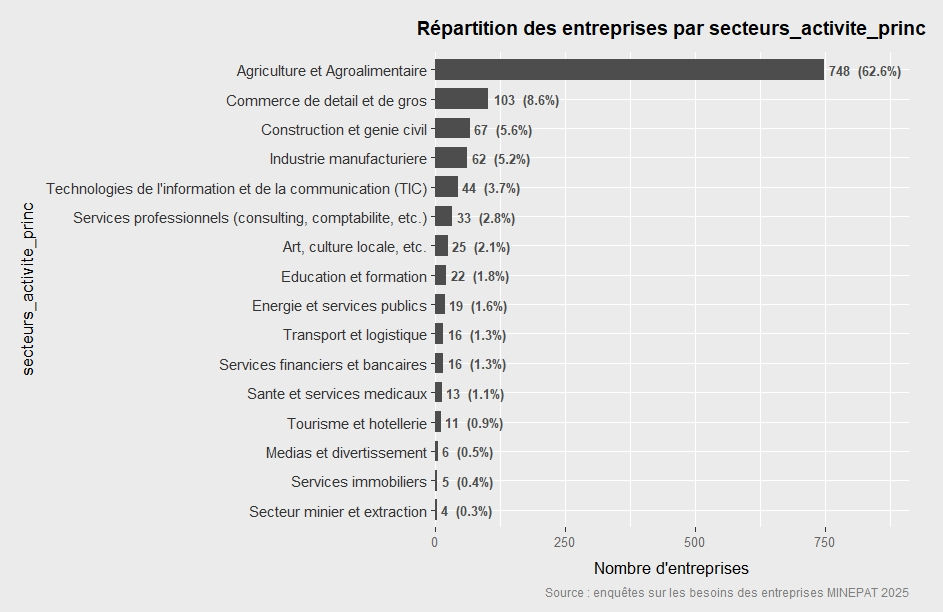
\includegraphics[width=\textwidth]{repartition_activite.jpeg}
        \caption{Répartition des entreprises par secteur d'activité}
        \label{fig:sous_fig_d}
    \end{subfigure}
    \hfill
    \begin{subfigure}[b]{0.52\textwidth}
        \centering
        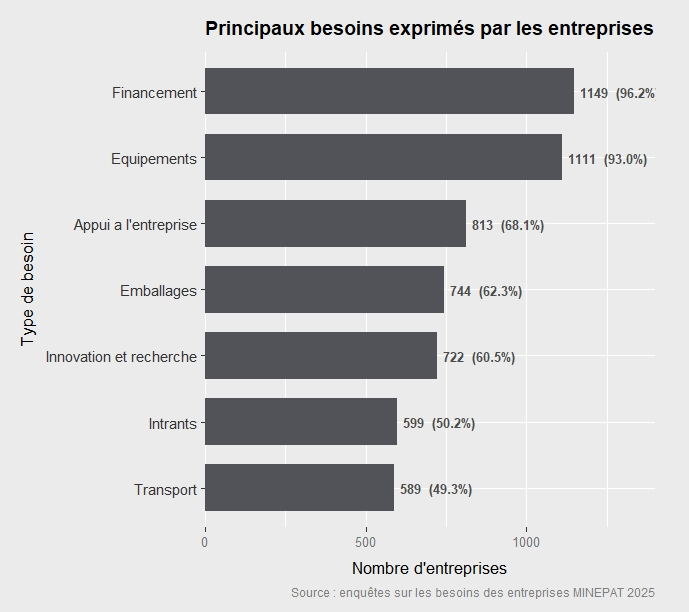
\includegraphics[width=\textwidth]{besoinsCorriges.jpeg}
        \caption{Répartition des besoins des entreprises}
        \label{fig:sous_fig_e}
    \end{subfigure}
    \caption{Répartition des entreprises selon leurs variables descriptives et leurs besoins (Total entreprises : 1194)}
    \label{fig:besoins_secteur_global}
\end{figure}
\vspace{6pt}

On observe très peu de grandes entreprises (1,3\%), tandis que plus de la moitié sont des petites entreprises (53,4\%). La région du Centre concentre le plus grand nombre d'entreprises (39,3\%), suivie du Littoral (17,8\%) — un constat qui interroge, la capitale économique se trouvant précisément dans cette dernière région. 62,6\% des entreprises relèvent du secteur Agriculture et Agroalimentaire, et les besoins les plus récurrents sont le financement (96,2\%) et les équipements (93,0\%). Les autres besoins, bien que moins fréquents, restent bien représentés dans l'échantillon.

\begin{frame}{Synthèse de l'analyse bivariée (test $\chi^2$ et $V$ de Cramér)}
    \begin{center}
        \scriptsize
        \renewcommand{\arraystretch}{1.2}
        \begin{tabular}{l|ccccc}
            \toprule
            \textbf{Besoins exprimés} & \textbf{Statut} & \textbf{Région} & \textbf{Ancien.} & \textbf{Secteur} & \textbf{Taille} \\
            \midrule
            Besoin en intrants & \cellcolor{green!15}0,11 & \cellcolor{green!15}0,16 & Non & \cellcolor{green!15}0,29 & Non \\
            \rowcolor{gray!5}
            Besoin en financement & Non & Non & Non & \cellcolor{green!15}0,17 & Non \\
            Besoin en emballages & \cellcolor{green!15}0,19 & \cellcolor{green!15}0,13 & Non & \cellcolor{blue!15}\textbf{0,51} & Non \\
            \rowcolor{gray!5}
            Besoin en transport & \cellcolor{green!15}0,21 & \cellcolor{green!15}0,16 & Non & \cellcolor{green!15}0,35 & Non \\
            Appui aux entreprises & \cellcolor{green!15}0,15 & \cellcolor{green!15}0,14 & \cellcolor{green!10}0,10 & Non & \cellcolor{green!10}0,11 \\
            \rowcolor{gray!5}
            Besoin en équipements & \cellcolor{green!15}0,23 & \cellcolor{green!15}0,15 & \cellcolor{green!10}0,11 & \cellcolor{blue!15}\textbf{0,45} & Non \\
            Innovation \& Recherche & \cellcolor{green!15}0,26 & \cellcolor{green!15}0,14 & \cellcolor{green!10}0,13 & \cellcolor{green!15}0,37 & Non \\
            \midrule
            \textbf{Significativité} & \textbf{6 / 7} & \textbf{6 / 7} & \textbf{3 / 7} & \textbf{6 / 7} & \textbf{1 / 7} \\
            \bottomrule
        \end{tabular}
    \end{center}
    \vfill
    \begin{itemize}
        \item \tiny \textbf{Légende :} les valeurs indiquent le $V$ de Cramér pour les tests significatifs ($p < 0,05$).
        \item \tiny \color{blue!80}\textbf{Bleu} : association très forte ($V > 0,40$). \color{black} | \color{gray}\textbf{Non} : test non significatif.
    \end{itemize}
\end{frame}

\begin{frame}{Principaux enseignements de l'analyse}
    \begin{itemize}
        \item \textbf{Le secteur d'activité : déterminant n°1}
        \begin{itemize}
            \item Influence fortement les besoins matériels : emballages ($V=0,51$) et équipements ($V=0,45$).
        \end{itemize}
        \vfill
        \item \textbf{L'universalité du besoin en financement}
        \begin{itemize}
            \item \alert{Exception statistique} : indépendant de la taille, de la région et de l'ancienneté ;
            \item Contrainte structurelle transversale à tout le tissu économique.
        \end{itemize}
        \vfill
        \item \textbf{Une logique de cycle de vie}
        \begin{itemize}
            \item Jeunes/petites structures : priorité à l'amorçage (équipements, appui institutionnel) ;
            \item Entreprises matures (20 ans et plus) : virage vers la compétitivité (innovation \& recherche).
        \end{itemize}
        \vfill
        \item \textbf{Des disparités régionales marquées}
        \begin{itemize}
            \item Besoins en transport et intrants prononcés dans les zones enclavées (Nord-Ouest, Est, Adamaoua).
        \end{itemize}
    \end{itemize}
\end{frame}

% ============================================================
\section{Résultat de l'analyse multidimensionnelle}
% ============================================================

\begin{frame}{Pipeline d'analyse}
    \centering
    \begin{tikzpicture}[
        node distance=0.6cm and 1.2cm,
        box/.style={rectangle, draw=primary, fill=primary!12,
            text width=2.5cm, align=center, rounded corners=4pt,
            minimum height=1.1cm, font=\small\bfseries},
        arrow/.style={->, very thick, color=primary},
        txtlabel/.style={font=\scriptsize\itshape, color=darkgray, align=center}
        ]
        \node[box] (acm) {ACM};
        \node[box, right=of acm] (cah) {CAH};
        \node[box, right=of cah] (afd) {AFD};
        \node[box, right=of afd, fill=secondary!20, draw=secondary] (plat)
        {Plateforme\\de mise en\\relation};

        \draw[arrow] (acm) -- (cah);
        \draw[arrow] (cah) -- (afd);
        \draw[arrow] (afd) -- (plat);

        \node[txtlabel, below=0.15cm of acm]
        {Réduction\\de dimension};
        \node[txtlabel, below=0.15cm of cah]
        {Partition en\\3 classes};
        \node[txtlabel, below=0.15cm of afd]
        {Validation \& \\prédiction};
        \node[txtlabel, below=0.15cm of plat]
        {Recommandation\\ciblée};
    \end{tikzpicture}

    \vspace{10pt}
    \begin{columns}[T]
        \begin{column}{0.3\textwidth}
            \begin{block}{\hfill ACM\hfill}
                \centering\scriptsize
                Variables qualitatives\\
                $\downarrow$\\
                Axes factoriels\\
                (DVS de $\mathbf{S}$)
            \end{block}
        \end{column}
        \begin{column}{0.3\textwidth}
            \begin{block}{\hfill CAH\hfill}
                \centering\scriptsize
                Coordonnées factorielles\\
                $\downarrow$\\
                Critère de Ward\\
                3 classes
            \end{block}
        \end{column}
        \begin{column}{0.3\textwidth}
            \begin{block}{\hfill AFD\hfill}
                \centering\scriptsize
                Classes connues\\
                $\downarrow$\\
                Critère de Fisher\\
                Règle de Bayes
            \end{block}
        \end{column}
    \end{columns}
\end{frame}

\begin{frame}{ACM — Analyse des Correspondances Multiples}
    \begin{columns}[T]
        \begin{column}{0.48\textwidth}
            \begin{block}{Principe}
                \begin{itemize}
                    \item Tableau disjonctif complet
                          $\mathbf{Z} \in \{0,1\}^{n \times K}$
                    \item Matrice des profils~:
                          $\mathbf{P} = \tfrac{1}{nQ}\mathbf{Z}$
                    \item Matrice à décomposer~:
                \end{itemize}
                \vspace{4pt}
                \[
                    \mathbf{S} = \mathbf{D}_r^{-1/2}
                    \!\left(\mathbf{P} - \mathbf{r}\mathbf{c}^{\top}\right)
                    \!\mathbf{D}_c^{-1/2}
                \]
            \end{block}
        \end{column}
        \begin{column}{0.48\textwidth}
            \begin{block}{DVS et projections}
                Décomposition~: $\mathbf{S} = \mathbf{U}\boldsymbol{\Sigma}\mathbf{V}^{\top}$
                \vspace{4pt}
                \begin{itemize}
                    \item Valeurs propres~:
                          $\lambda_s = \sigma_s^2$
                    \item Coordonnées individus~:
                          \[
                              \mathbf{F} =
                              \mathbf{D}_r^{-1/2}\mathbf{U}\boldsymbol{\Sigma}
                          \]
                    \item Coordonnées modalités~:
                          \[
                              \mathbf{G} =
                              \mathbf{D}_c^{-1/2}\mathbf{V}\boldsymbol{\Sigma}
                          \]
                \end{itemize}
            \end{block}
        \end{column}
    \end{columns}
    \vspace{6pt}
    \begin{exampleblock}{Propriété barycentrique}
        Les individus sont représentés au barycentre de leurs modalités~;
        les modalités au barycentre des individus qui les possèdent.
    \end{exampleblock}
\end{frame}

\begin{frame}{ACM : objectif et choix des axes (éboulis des VP)}
    \begin{columns}[c]
        \begin{column}{0.55\textwidth}
            \begin{figure}
                \centering
                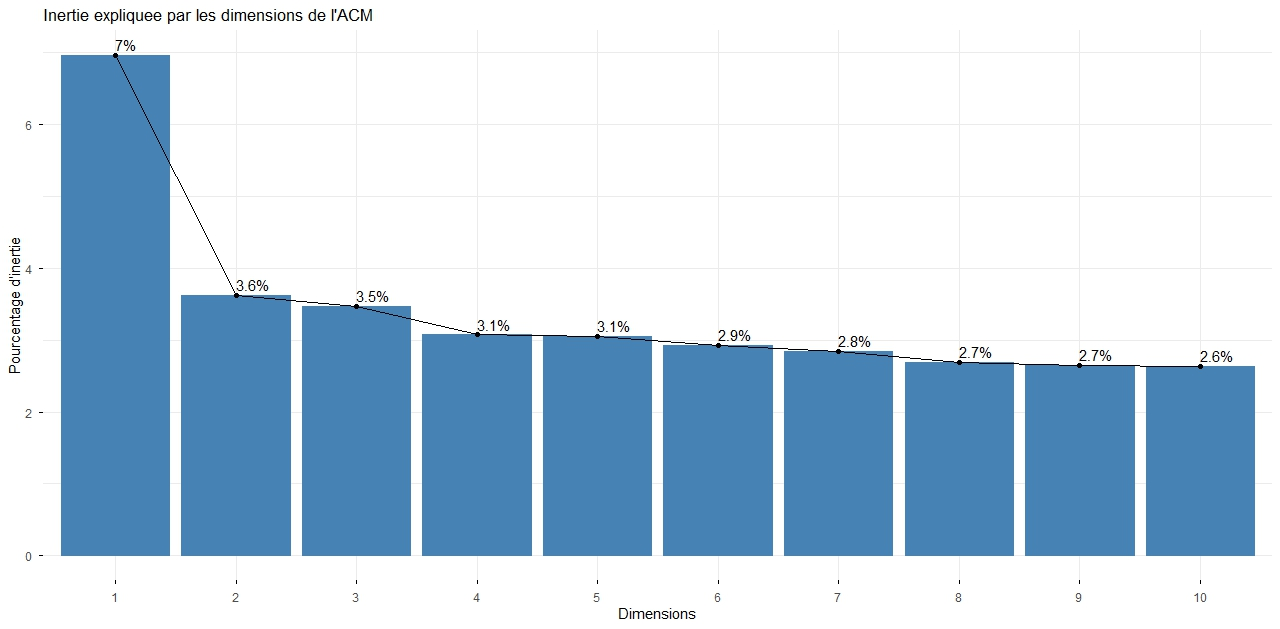
\includegraphics[width=\textwidth]{contributionValeursPropres.jpeg}
                \caption{\label{fig:acm_vp}Éboulis des valeurs propres}
            \end{figure}
        \end{column}
        \begin{column}{0.42\textwidth}
            \textbf{Objectif de l'ACM :}
            \begin{itemize}
                \item Synthétiser le nuage d'entreprises à partir des variables qualitatives (\texttt{FactoMineR}).
            \end{itemize}
            \vfill
            \textbf{Sélection du nombre d'axe factoriel}
            \begin{itemize}
                \item Utilisation des valeurs propres corrigées de Benzecri;
                \item $\hat{\lambda}_s =
                \left(\frac{p}{p-1}\right)^2
                \left(\lambda_s - \frac{1}{p}\right)^2
                \quad \text{pour } \lambda_s > \frac{1}{p}
                \label{eq:correction_benzecri}$
                \item $
                	\tilde{\tau}_s =
                	\frac{\hat{\lambda}_s}{\displaystyle\sum_{s'} \hat{\lambda}_{s'}}
                	\times 100
                	\label{eq:tau_corrige}
                $
                \item $\sum_{i=1}^{5}\tilde{\tau_{si}}=88,74\%$
                
            \end{itemize}
        \end{column}
    \end{columns}
\end{frame}

\begin{frame}{Projection des modalités (axes 1 \& 2)}
    \begin{center}
        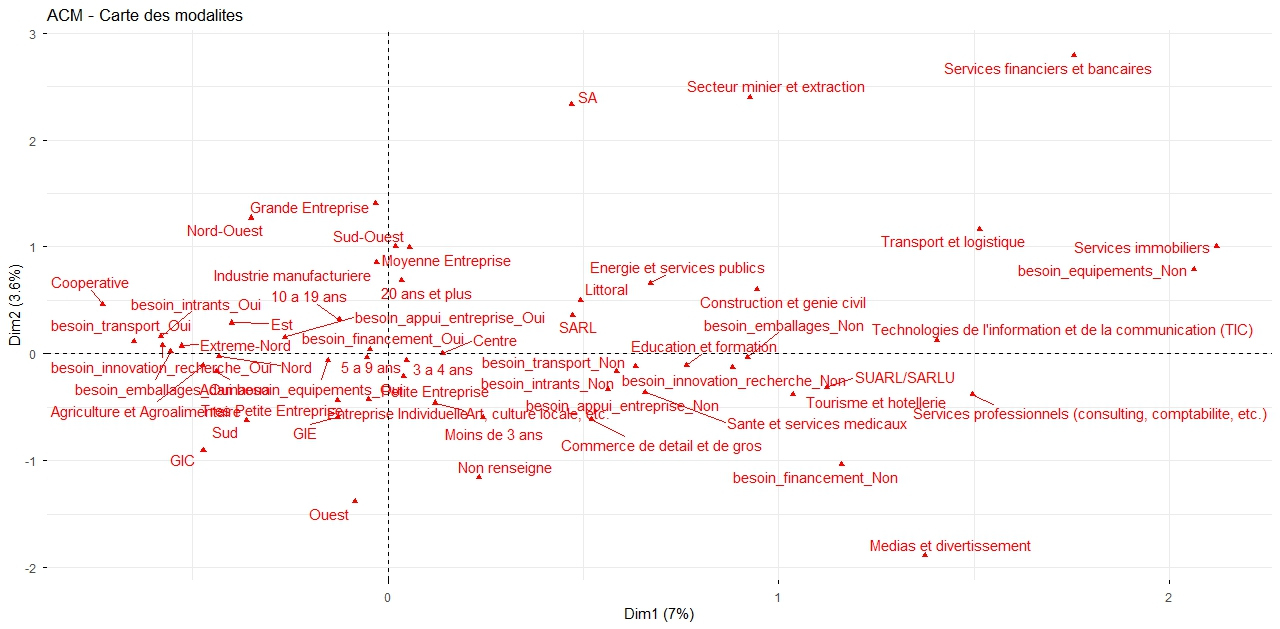
\includegraphics[width=0.7\textwidth]{projectionDesCategories.jpeg}
    \end{center}
    \begin{block}{Interprétation des axes}
        \begin{itemize}
            \item \textbf{Axe 1 (horizontal)} : oppose les entreprises du tertiaire à celles du secteur primaire (nature des besoins et secteurs) ;
            \item \textbf{Axe 2 (vertical)} : discrimine les structures selon leur \textbf{statut juridique} et leur \textbf{taille} ;
            \item \alert{\textbf{Fait marquant}} : le \textit{besoin en financement} se situe quasi au centre $\rightarrow$ \textbf{besoin transversal} à toutes les entreprises.
        \end{itemize}
    \end{block}
\end{frame}

\begin{frame}{Contributions à l'Axe 1 : besoins opérationnels (7\% d'inertie)}
    \begin{columns}[c]
        \begin{column}{0.5\textwidth}
            \begin{figure}
                \centering
                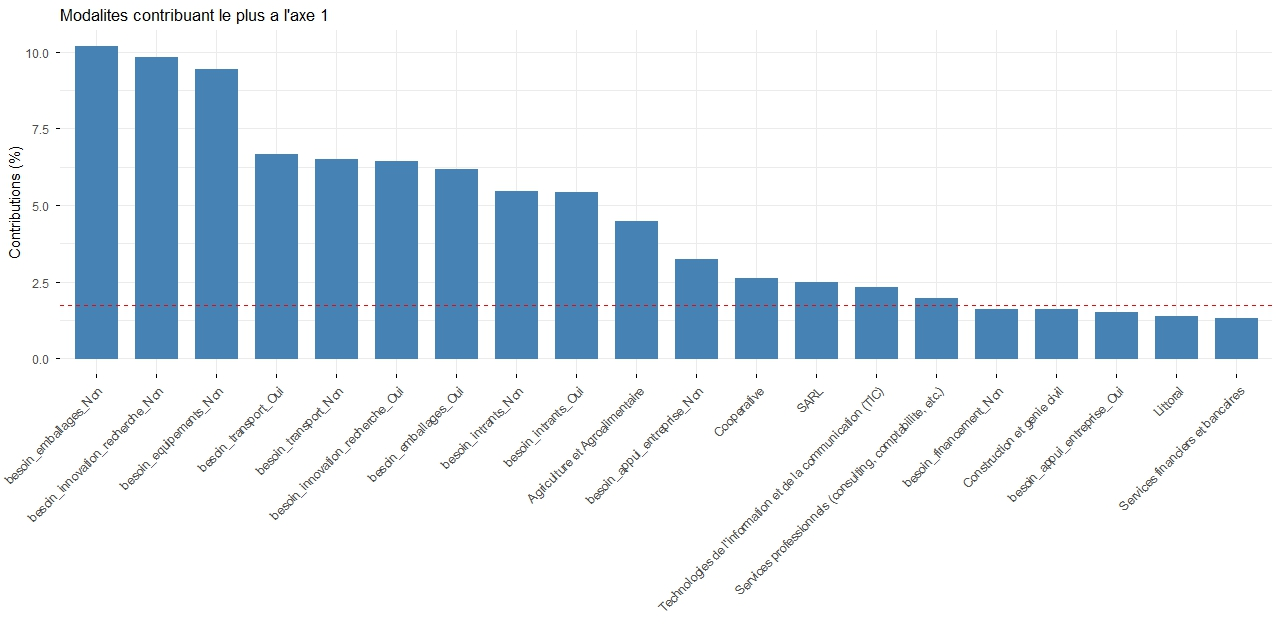
\includegraphics[width=\textwidth]{contributionCategoriesAlAxe1.jpeg}
                \caption{Contributions à l'Axe 1}
            \end{figure}
        \end{column}
        \begin{column}{0.48\textwidth}
            \textbf{Un axe dicté par les besoins matériels et techniques :}
            \begin{itemize}
                \item \textbf{Top 3 des modalités (>10\% chacune)} :
                \begin{itemize}
                    \item \texttt{besoin\_emballages\_Non}
                    \item \texttt{besoin\_innovation\_Non}
                    \item \texttt{besoin\_equipements\_Non}
                \end{itemize}
                \item \textbf{Effet miroir (5\% à 7\%)} : présence vs absence des besoins logistiques (transport, emballages, innovation).
            \end{itemize}
            \begin{exampleblock}{Synthèse Axe 1}
                Dichotomie nette entre la présence et l'absence de besoins matériels et technologiques.
            \end{exampleblock}
        \end{column}
    \end{columns}
\end{frame}

\begin{frame}{Contributions à l'Axe 2 : structure institutionnelle (3,6\% d'inertie)}
    \begin{columns}[c]
        \begin{column}{0.5\textwidth}
            \begin{figure}
                \centering
                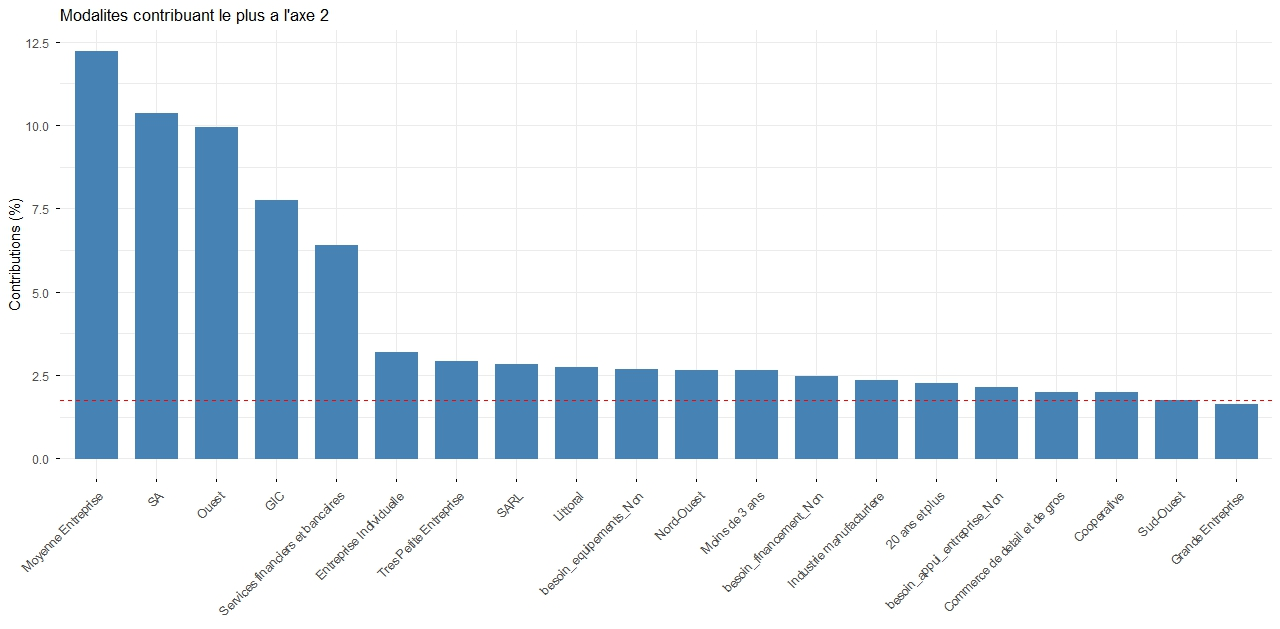
\includegraphics[width=\textwidth]{contributionCategorieALAxe2.jpeg}
                \caption{Contributions à l'Axe 2}
            \end{figure}
        \end{column}
        \begin{column}{0.48\textwidth}
            \textbf{Rupture totale : un axe purement statutaire et géographique}
            \begin{itemize}
                \item \textbf{5 piliers majeurs} (au-dessus du seuil) :
                \begin{enumerate}
                    \item Moyenne entreprise ($\sim$12\%)
                    \item Forme juridique SA ($\sim$10,5\%)
                    \item Région de l'Ouest ($\sim$10\%)
                    \item Statut de GIC ($\sim$7,5\%)
                    \item Secteur Finances/Banques ($\sim$6,5\%)
                \end{enumerate}
                \item L'âge et les besoins opérationnels n'ont ici aucune influence.
            \end{itemize}
            \begin{exampleblock}{Synthèse Axe 2}
                Capte spécifiquement le niveau de formalisation légale et la structuration des entités.
            \end{exampleblock}
        \end{column}
    \end{columns}
\end{frame}

\begin{frame}{CAH — Classification Ascendante Hiérarchique}
    \begin{columns}[T]
        \begin{column}{0.52\textwidth}
            \begin{block}{Algorithme de Ward}
                Fusion itérative des paires minimisant la
                perte d'inertie inter-classes~:
                \[
                    \Delta(C_a, C_b)
                    = \frac{n_a \cdot n_b}{n_a + n_b}
                      \left\|\bar{x}_a - \bar{x}_b\right\|^2
                \]
                Distance entre individus (espace ACM)~:
                \[
                    d(\omega_i, \omega_j)
                    = \sqrt{\sum_{s=1}^{q}(F_{is} - F_{js})^2}
                \]
            \end{block}
        \end{column}
        \begin{column}{0.44\textwidth}
            \begin{exampleblock}{Choix de 3 classes}
                \begin{itemize}
                    \item Choix définie pour une meilleure visibilité  ;
                    \item Meilleure répartition des entreprises dans les classes;
                    \item Trois profils distincts~:
                          \begin{itemize}
                              \item[\textbullet] Acteurs agro-productifs émergents
                              \item[\textbullet]  Opérateurs
                              financiers et autres services établis
                              \item[\textbullet]  Petites entreprises multiple-sectorielles
                          \end{itemize}
                \end{itemize}
            \end{exampleblock}
        \end{column}
    \end{columns}
\end{frame}

\begin{frame}{CAH : méthodologie et choix de la partition}
    \begin{columns}[c]
        \begin{column}{0.52\textwidth}
            \begin{figure}
                \centering
                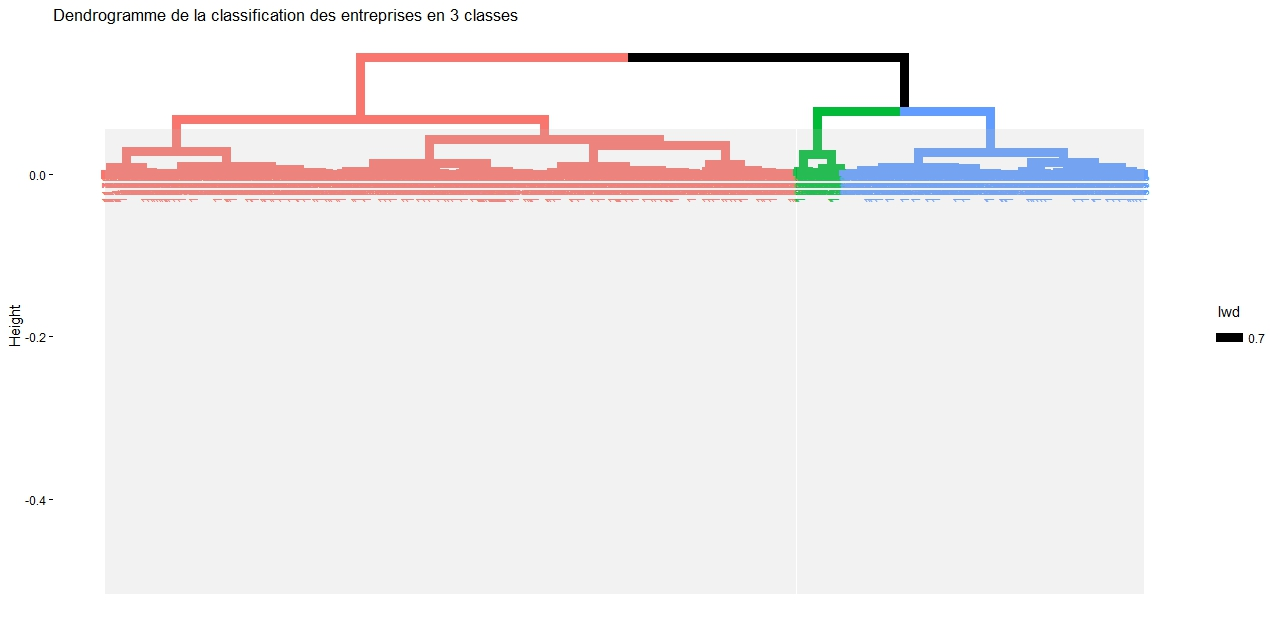
\includegraphics[width=\textwidth]{dendrogramme.jpeg}
                \caption{Dendrogramme (méthode de Ward)}
            \end{figure}
        \end{column}
        \begin{column}{0.45\textwidth}
            \textbf{Approche méthodologique :}
            \begin{itemize}
                \item CAH basée sur les coordonnées factorielles de l'ACM ;
                \item Critère de Ward (minimisation de la perte d'inertie intra-classe).
            \end{itemize}
            \vfill
            \textbf{Choix de 3 classes :}
            \begin{itemize}
                \item Retenu pour sa lisibilité opérationnelle et le saut d'inertie observé au dendrogramme.
            \end{itemize}
        \end{column}
    \end{columns}
\end{frame}

\begin{frame}{Projection de la partition sur le premier plan factoriel}
    \begin{center}
        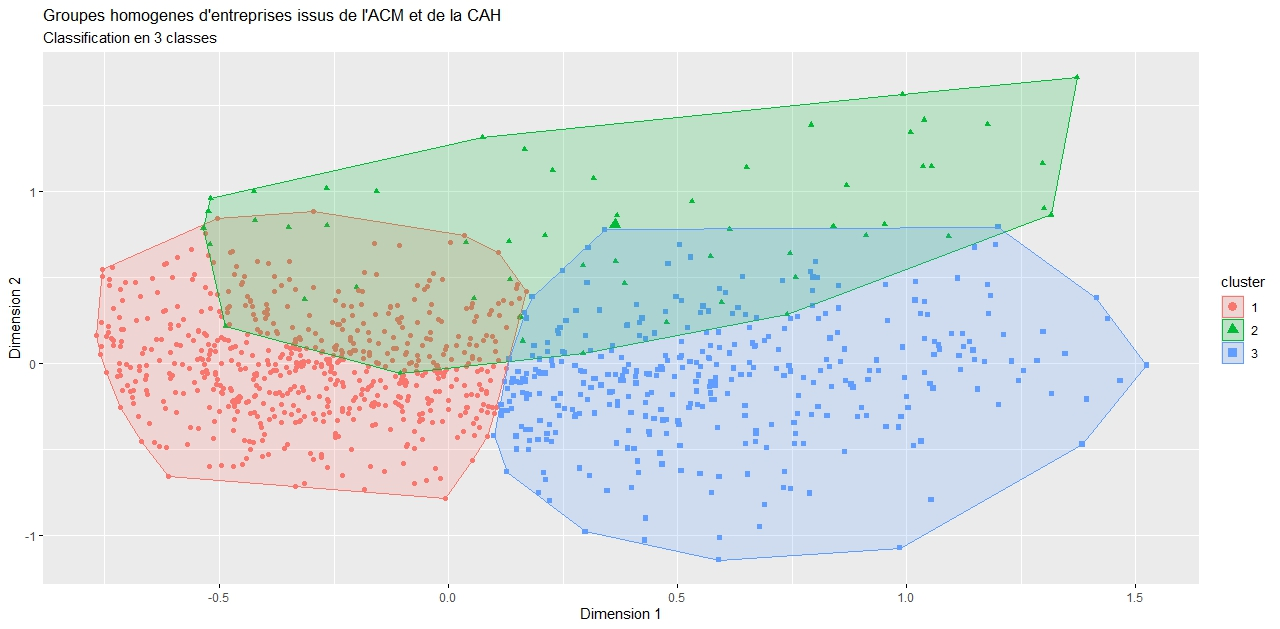
\includegraphics[width=0.68\textwidth]{CAH.jpeg}
    \end{center}
    \begin{block}{Validation de la cohérence des groupes}
        \begin{itemize}
            \item Les trois classes occupent des \textbf{zones bien distinctes} du plan factoriel ;
            \item Excellente homogénéité intra-classe et séparation inter-classes satisfaisante ;
            \item Le croisement ACM-CAH permet de segmenter efficacement le tissu économique.
        \end{itemize}
    \end{block}
\end{frame}

\begin{frame}{Profil dominant des trois classes obtenues}
    \begin{center}
        \scriptsize
        \renewcommand{\arraystretch}{1.2}
        \begin{tabular}{l|c|c|c}
            \toprule
            \textbf{Caractéristiques} & \textbf{Classe 1 ($63,1\,\%$)} & \textbf{Classe 2 ($4,8\,\%$)} & \textbf{Classe 3 ($32,2\,\%$)} \\
            \textbf{Dominantes} & \textit{753 entreprises} & \textit{57 entreprises} & \textit{384 entreprises} \\
            \midrule
            \textbf{Ancienneté} & 5 à 9 ans ($40,2\,\%$) & Plus de 20 ans ($26,4\,\%$) & 5 à 9 ans ($38,8\,\%$) \\
            \rowcolor{gray!5}
            \textbf{Secteur} & \textbf{Agri. / Agroalim.} ($81,1\,\%$) & Services Fin. ($24,6\,\%$) & Agri. / Agroalim. ($31,2\,\%$) \\
            \textbf{Région} & Centre ($36,3\,\%$) & Centre ($45,5\,\%$) & Centre ($45,6\,\%$) \\
            \rowcolor{gray!5}
            \textbf{Taille} & \alert{\textbf{Petite Entr.}} ($52,5\,\%$) & \alert{\textbf{Moyenne Entr.}} ($54,4\,\%$) & \alert{\textbf{Petite Entr.}} ($59,6\,\%$) \\
            \bottomrule
        \end{tabular}
    \end{center}
    \begin{block}{Résumé}
        \begin{itemize}
            \tiny
            \item \textbf{Classe 1 (cœur de cible)} : majorité d'agro-PME installées en phase de consolidation (5-9 ans).
            \item \textbf{Classe 2 (grands comptes)} : entreprises matures, plus grandes, orientées vers le secteur financier.
            \item \textbf{Classe 3 (profil intermédiaire)} : petites entreprises du Centre, diversifiées mais à fort ancrage agricole.
        \end{itemize}
    \end{block}
\end{frame}

\begin{frame}{AFD — Vecteurs discriminants (Fisher, 1936)}
    \begin{columns}[T]
        \begin{column}{0.48\textwidth}
            \begin{block}{Décomposition de la variance}
                \[
                    \mathbf{T} = \underbrace{\mathbf{W}}_{\text{intra}}
                               + \underbrace{\mathbf{B}}_{\text{inter}}
                \]
                Critère de Fisher~:
                \[
                    \mathbf{a}^* =
                    \underset{\mathbf{a}}{\arg\max}\;
                    \frac{\mathbf{a}^{\top}\mathbf{B}\,\mathbf{a}}
                         {\mathbf{a}^{\top}\mathbf{W}\,\mathbf{a}}
                \]
            \end{block}
        \end{column}
        \begin{column}{0.48\textwidth}
            \begin{block}{Problème aux valeurs propres}
                \[
                    \mathbf{W}^{-1}\mathbf{B}\,\mathbf{a}_s
                    = \lambda_s\,\mathbf{a}_s
                \]
                Part de discrimination de l'axe $s$~:
                \[
                    \tau_s =
                    \frac{\lambda_s}{\sum_{s'} \lambda_{s'}}
                \]
                \vspace{2pt}
                \textbf{Résultat obtenu~:}\\
                LD1 : 58,6\,\% \quad LD2 : 41,4\,\%\\
                $\Rightarrow$ \textbf{100\,\% en 2 axes}
            \end{block}
        \end{column}
    \end{columns}
\end{frame}

\begin{frame}{AFD — Règle de classification bayésienne}
    \begin{block}{Score discriminant de Bayes}
        \[
            \delta_c(\mathbf{x}_i)
            = \mathbf{x}_i^{\top}\boldsymbol{\Sigma}^{-1}\boldsymbol{\mu}_c
            - \tfrac{1}{2}\,\boldsymbol{\mu}_c^{\top}
              \boldsymbol{\Sigma}^{-1}\boldsymbol{\mu}_c
            + \log(\pi_c)
        \]
    \end{block}
    \vspace{4pt}
    \begin{columns}[T]
        \begin{column}{0.48\textwidth}
            \begin{block}{Règle de décision}
                \[
                    \hat{c}(\mathbf{x}_i)
                    = \underset{c}{\arg\max}\;
                      \delta_c(\mathbf{x}_i)
                \]
                \small Implémenté via \texttt{MASS::lda()} en R.\\
                La décision repose sur les \textbf{probabilités
                a posteriori} $P(\mathcal{C}_c \mid \mathbf{x}_i)$.
            \end{block}
        \end{column}
        \begin{column}{0.48\textwidth}
            \begin{exampleblock}{Interprétation géométrique}
                Équivalent à affecter l'individu à la classe dont
                le centroïde est le plus proche au sens de la
                \textbf{distance de Mahalanobis} corrigée des
                probabilités a priori $\pi_c = n_c / n$.
            \end{exampleblock}
        \end{column}
    \end{columns}
\end{frame}

\begin{frame}{AFD : validation de la séparation des classes}
    \begin{columns}[c]
        \begin{column}{0.55\textwidth}
            \begin{figure}
                \centering
                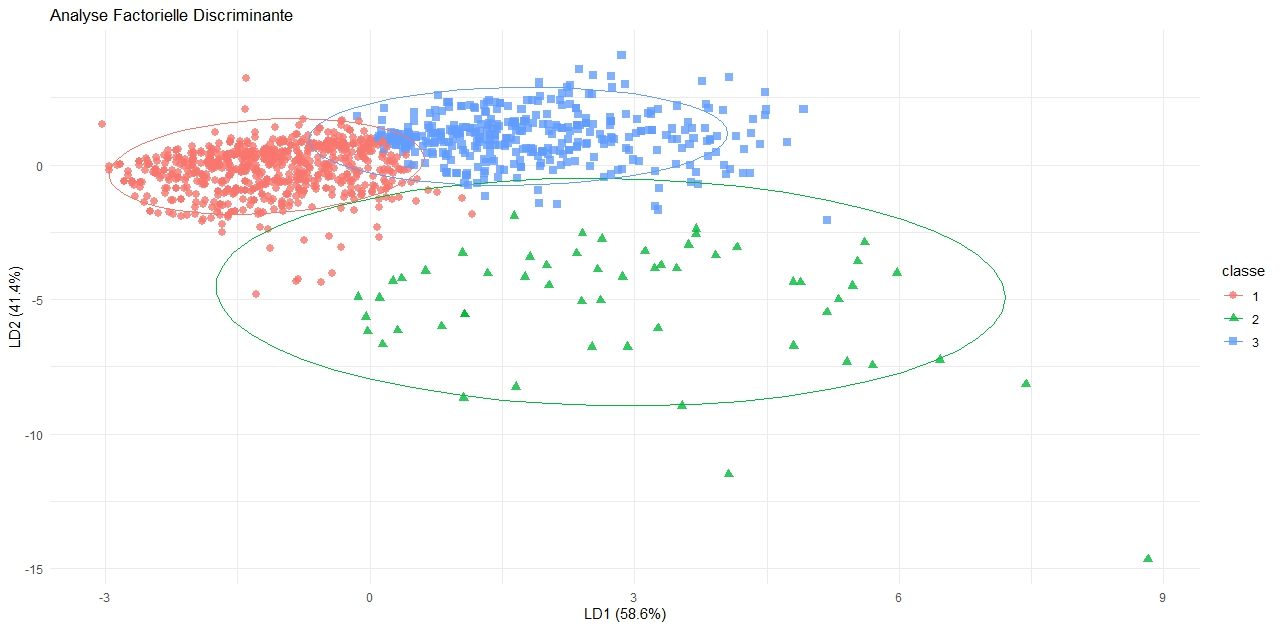
\includegraphics[width=\textwidth]{AFDProjectionDesObservations.jpeg}
                \caption{Projection des observations sur les axes discriminants}
            \end{figure}
        \end{column}
        \begin{column}{0.42\textwidth}
            \textbf{Pouvoir discriminant total :}
            \begin{itemize}
                \item \alert{\textbf{100\,\% de l'inertie}} captés par le premier plan factoriel ;
                \item \textbf{LD1} : 58,6\,\% de séparation ;
                \item \textbf{LD2} : 41,4\,\% de séparation.
            \end{itemize}
            \vfill
            \textbf{Pertinence statistique :}
            \begin{itemize}
                \item Séparation globale optimale des trois classes ;
                \item Ellipses de confiance à 95\,\% bien distinctes ;
                \item \textit{Note} : léger chevauchement mineur entre les classes 1 et 3.
            \end{itemize}
        \end{column}
    \end{columns}
\end{frame}

\begin{frame}{Coefficients des variables sur les axes LD1 et LD2}
    \begin{columns}[c]
        \begin{column}{0.48\textwidth}
            \begin{center}
                \footnotesize
                \renewcommand{\arraystretch}{1.2}
                \begin{tabular}{l|rr}
                    \toprule
                    \textbf{Variables (ACM)} & \textbf{LD1} & \textbf{LD2} \\
                    \midrule
                    \textbf{Dim1} & \cellcolor{red!15}\textbf{3,4117} & 0,8420 \\
                    \rowcolor{gray!5}
                    \textbf{Dim2} & 0,5020 & \cellcolor{blue!15}\textbf{$-$2,8215} \\
                    \textbf{Dim3} & 1,0018 & \cellcolor{blue!15}\textbf{$-$2,3454} \\
                    \rowcolor{gray!5}
                    \textbf{Dim4} & 0,7551 & \cellcolor{blue!15}\textbf{$-$2,1043} \\
                    \textbf{Dim5} & $-$0,5523 & 1,0850 \\
                    \bottomrule
                \end{tabular}
            \end{center}
        \end{column}
        \begin{column}{0.5\textwidth}
            \begin{block}{Fonction LD1 : axe principal}
                \begin{itemize}
                    \scriptsize
                    \item Largement dominée par \textbf{Dim1} (3,41) ;
                    \item Dimension de discrimination la plus puissante issue des besoins de l'ACM.
                \end{itemize}
            \end{block}
            \begin{block}{Fonction LD2 : axe secondaire}
                \begin{itemize}
                    \scriptsize
                    \item Oppose fortement \textbf{Dim2, Dim3 et Dim4} (coefficients négatifs marqués) à Dim1 et Dim5 ;
                    \item Capte une variation orthogonale pour affiner la séparation des groupes restants.
                \end{itemize}
            \end{block}
        \end{column}
    \end{columns}
\end{frame}

\begin{frame}{Indicateurs de performance du modèle discriminant}
    \begin{center}
        \small
        \renewcommand{\arraystretch}{1.2}
        \begin{tabular}{l|c|l}
            \toprule
            \textbf{Indicateur} & \textbf{Valeur} & \textbf{Interprétation} \\
            \midrule
            \textbf{Accuracy (précision)} & \textbf{97,24\,\%} & Classification globale excellente [96,1\,\%~--~98,1\,\%] \\
            \rowcolor{gray!5}
            \textbf{Kappa de Cohen} & \textbf{0,9435} & Accord quasi-parfait (corrige l'effet du hasard) \\
            \textbf{Accuracy Null} & 63,07\,\% & Performance d'un classifieur naïf \\
            \rowcolor{gray!5}
            \textbf{Gain de performance} & \alert{\textbf{+34,17\,\%}} & Apport réel et massif du modèle discriminant \\
            \bottomrule
        \end{tabular}
    \end{center}
    \vfill
    \begin{block}{Significativité statistique ($p < 0,05$)}
        \begin{itemize}
            \small
            \item \textbf{$p$-valeur globale} : $5,16 \times 10^{-183} \rightarrow$ modèle infiniment supérieur à un choix aléatoire ;
            \item \textbf{Test de McNemar} ($p = 8,50 \times 10^{-7}$) : erreurs du modèle non uniformément réparties entre les classes.
        \end{itemize}
    \end{block}
\end{frame}

% ============================================================
%  NOUVELLE SECTION — PRÉSENTATION DE L'APPLICATION
%  C'est ici que se fait le pont entre l'analyse statistique
%  et le livrable applicatif : à insérer avant la conclusion.
% ============================================================
\section{Présentation de l'application « Business Partnership »}

\begin{frame}{De l'analyse à l'action : la plateforme Business Partnership}
    Les profils de besoins identifiés par le pipeline ACM $\to$ CAH $\to$ AFD alimentent directement la logique de recommandation de la plateforme développée pour le MINEPAT/DAPE.
    \vspace{6pt}
    \begin{block}{Ce que fait la plateforme}
        \begin{itemize}
            \item Recense les entreprises et les besoins/offres qu'elles déclarent ;
            \item Met automatiquement en relation les entreprises dont l'offre répond à un besoin exprimé par une autre ;
            \item Fournit aux agents de la DAPE un outil de pilotage et de suivi des mises en relation.
        \end{itemize}
    \end{block}
    \begin{alertblock}{Positionnement}
        Une approche par \textbf{système à base de connaissances} (cf. état de l'art) : le matching s'appuie sur la correspondance explicite entre besoins déclarés et offres déclarées, plutôt que sur un historique de comportements.
    \end{alertblock}
\end{frame}

\begin{frame}{Architecture technique}
    \centering
    \begin{tikzpicture}[
        node distance=0.5cm and 1.0cm,
        layer/.style={rectangle, draw=primary, fill=primary!10,
            text width=3.6cm, align=center, rounded corners=4pt,
            minimum height=1.3cm, font=\small\bfseries},
        arrow/.style={->, very thick, color=primary}
        ]
        \node[layer] (front) {Frontend\\\footnotesize Templates Django + Bootstrap};
        \node[layer, below=of front, fill=secondary!15, draw=secondary] (back) {Backend\\\footnotesize Django (vues, formulaires, ORM)};
        \node[layer, below=of back] (algo) {Moteur de matching\\\footnotesize \texttt{annotate()} / \texttt{Count()}};
        \node[layer, below=of algo, fill=successgreen!15, draw=successgreen] (db) {Base de données\\\footnotesize Modèle dimensionnel \texttt{BesoinOffreEntreprise}};

        \draw[arrow] (front) -- (back);
        \draw[arrow] (back) -- (algo);
        \draw[arrow] (algo) -- (db);
    \end{tikzpicture}
    \vspace{8pt}

    \small Déploiement~: hébergement du backend Django et du frontend sur \textbf{Render} \hfill \textit{(cf. guide de déploiement)}
\end{frame}

\begin{frame}{Modèle de données et algorithme de mise en relation}
    \begin{columns}[T]
        \begin{column}{0.5\textwidth}
            \begin{block}{Modèle en étoile}
                \begin{itemize}
                    \item Table de faits~: \texttt{BesoinOffreEntreprise} ;
                    \item Dimensions~: Entreprise, Secteur, Région, Type de besoin/offre ;
                    \item Repose sur les mêmes principes MERISE que la base d'analyse.
                \end{itemize}
            \end{block}
        \end{column}
        \begin{column}{0.48\textwidth}
            \begin{exampleblock}{Principe du matching}
                \begin{enumerate}
                    \item Une entreprise A déclare un besoin ;
                    \item Le moteur recherche les entreprises B ayant déclaré l'offre correspondante ;
                    \item Les résultats sont classés par nombre de correspondances (\texttt{Count}) ;
                    \item Les meilleurs partenaires sont proposés à l'entreprise A.
                \end{enumerate}
            \end{exampleblock}
        \end{column}
    \end{columns}
\end{frame}

\begin{frame}{Aperçu de l'interface — Tableau de bord}
    \centering
    % Remplacez les deux lignes ci-dessous par :
    % \includegraphics[width=0.48\textwidth]{dashboard.png}
    \screenshotplaceholder[6.2cm]{4.2cm}{Capture d'écran\\Tableau de bord entreprise\\\texttt{[dashboard.png]}}
    \hspace{4pt}
    \screenshotplaceholder[6.2cm]{4.2cm}{Capture d'écran\\Liste des besoins déclarés\\\texttt{[besoins\_list.png]}}
    \vspace{8pt}

    \footnotesize \textit{Emplacements réservés — insérer vos captures d'écran réelles ici.}
\end{frame}

\begin{frame}{Aperçu de l'interface — Fiche entreprise et mise en relation}
    \centering
    % Remplacez les deux lignes ci-dessous par :
    % \includegraphics[width=0.48\textwidth]{fiche_entreprise.png}
    \screenshotplaceholder[6.2cm]{4.2cm}{Capture d'écran\\Fiche entreprise\\\texttt{[fiche\_entreprise.png]}}
    \hspace{4pt}
    \screenshotplaceholder[6.2cm]{4.2cm}{Capture d'écran\\Résultats de mise en relation\\\texttt{[matching\_results.png]}}
    \vspace{8pt}

    \footnotesize \textit{Emplacements réservés — insérer vos captures d'écran réelles ici.}
\end{frame}

\begin{frame}{Accéder à la plateforme}
    \centering
    \vspace{4pt}
    {\Large \textbf{Démonstration en direct}}
    \vspace{10pt}

    \begin{columns}[c]
        \begin{column}{0.55\textwidth}
            \begin{block}{Lien d'accès}
                % Remplacez l'URL ci-dessous par l'adresse réelle de déploiement Render
                \href{https://business-partnership.onrender.com}{\Large\textbf{business-partnership.onrender.com}}
                \vspace{6pt}

                \small Identifiants de démonstration~:\\
                \texttt{login : demo@minepat.cm}\\
                \texttt{mot de passe : ********}
            \end{block}
        \end{column}
        \begin{column}{0.4\textwidth}
            \centering
            % Remplacez par : \includegraphics[width=3cm]{qrcode.png}
            \screenshotplaceholder[3.2cm]{3.2cm}{QR CODE\\\texttt{[qrcode.png]}}
        \end{column}
    \end{columns}
    \vspace{8pt}
    \footnotesize \textit{Scannez le QR code ou cliquez sur le lien pour explorer l'application.}
\end{frame}

% ============================================================
\section{Limites et perspectives}
% ============================================================

\begin{frame}{Limites et perspectives}
    \begin{columns}[T]
        \begin{column}{0.48\textwidth}
            \begin{alertblock}{Limites}
                \begin{itemize}
                    \item Échantillon limité aux entreprises ayant répondu à l'enquête ;
                    \item Classe 2 sous-représentée (4,8\,\%, 57 entreprises) — précision moindre pour ce profil ;
                    \item Matching fondé sur un simple comptage de correspondances, sans pondération des besoins prioritaires ;
                    \item Sécurité applicative encore basique (authentification simple).
                \end{itemize}
            \end{alertblock}
        \end{column}
        \begin{column}{0.48\textwidth}
            \begin{exampleblock}{Perspectives}
                \begin{itemize}
                    \item Introduire une pondération/similarité (approche hybride avec filtrage collaboratif) ;
                    \item Étendre la collecte à davantage d'entreprises pour rééquilibrer les classes ;
                    \item Ajouter un tableau de bord analytique pour le pilotage MINEPAT ;
                    \item Suivre les mises en relation effectivement abouties (retour terrain).
                \end{itemize}
            \end{exampleblock}
        \end{column}
    \end{columns}
\end{frame}

% ============================================================
\section{Conclusion}
% ============================================================

\begin{frame}{Conclusion}
    \begin{block}{Ce que ce travail apporte}
        Ce mémoire propose une démarche intégrée, de la
        \textbf{collecte des données terrain} à la
        \textbf{conception d'un outil numérique opérationnel},
        pour répondre à un besoin institutionnel réel du MINEPAT~:
        mieux connaître les entreprises camerounaises pour
        mieux les soutenir.
    \end{block}
    \vspace{10pt}
    \begin{columns}[T]
        \begin{column}{0.48\textwidth}
            \begin{exampleblock}{Contributions méthodologiques}
                Pipeline ACM $\to$ CAH $\to$ AFD appliqué à des
                données qualitatives d'enquête à grande échelle.
                Modèle de classification atteignant
                \textbf{97,24\,\%} de précision.
            \end{exampleblock}
        \end{column}
        \begin{column}{0.48\textwidth}
            \begin{exampleblock}{Contributions opérationnelles}
                Plateforme gouvernementale de cartographie
                et de mise en relation, directement utilisable
                par les agents de la DAPE-MINEPAT.
            \end{exampleblock}
        \end{column}
    \end{columns}
    \vspace{12pt}
    \centering
    \Large\textcolor{primary}{\textbf{Merci de votre attention}}\\[6pt]
    \normalsize\textcolor{darkgray}{Questions et remarques bienvenues}
\end{frame}

\end{document}
